\chapter{youBot placing experiment}
\section{Deliverables 6.2}
\textbf{Update your previous week’s report and include the following:}

\subsection{If necessary, rerun your experiment according to the feedback in class and describe how the new run improves on the previous run.}
We were not asked to rerun the experiment.

\subsection{Find suitable statistical techniques for analyzing the experimental results (using what you’ve learned during the LEGO experiment) and answer the following questions:}


\begin{figure}[ht!]
	\centering
	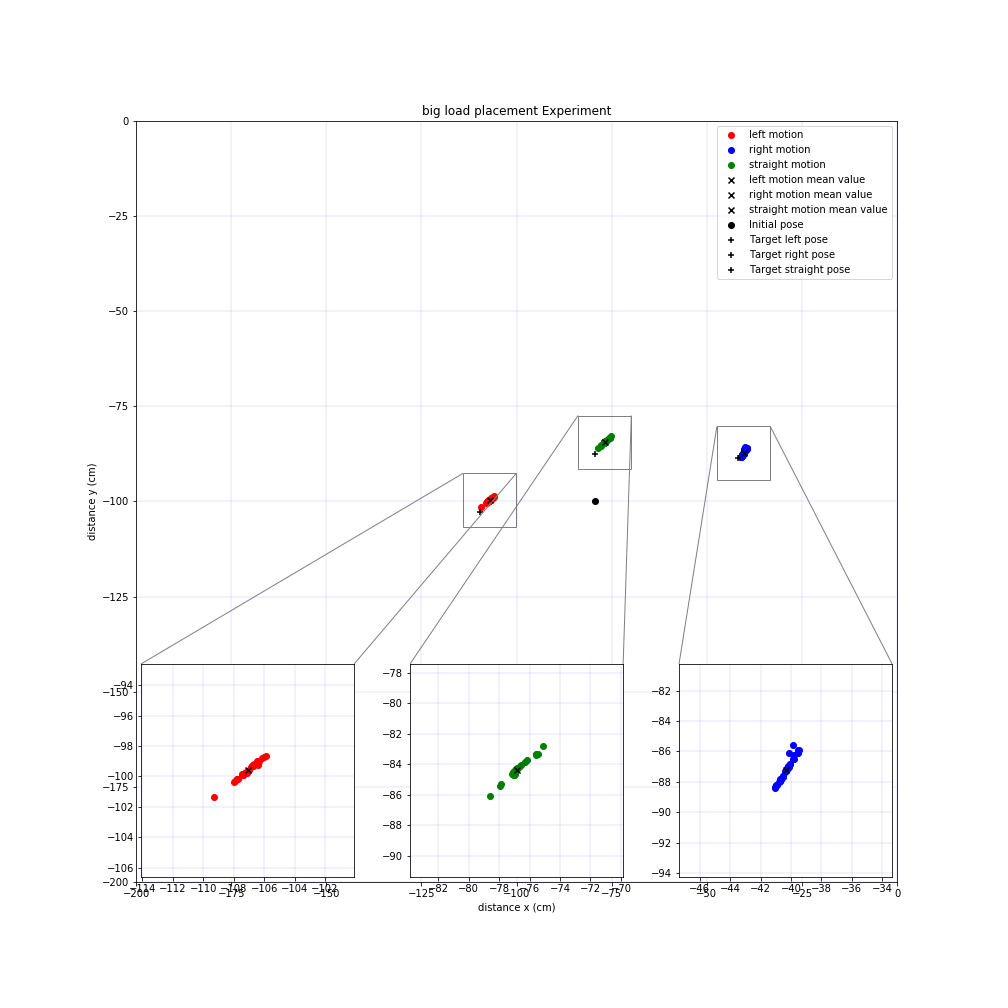
\includegraphics[width=0.6\linewidth]{images/combinedbig}
	\caption{Results of the Big Load Placement Experiment}
	\label{fig:combinedbig}
\end{figure}
\begin{figure}[ht!]
	\centering
	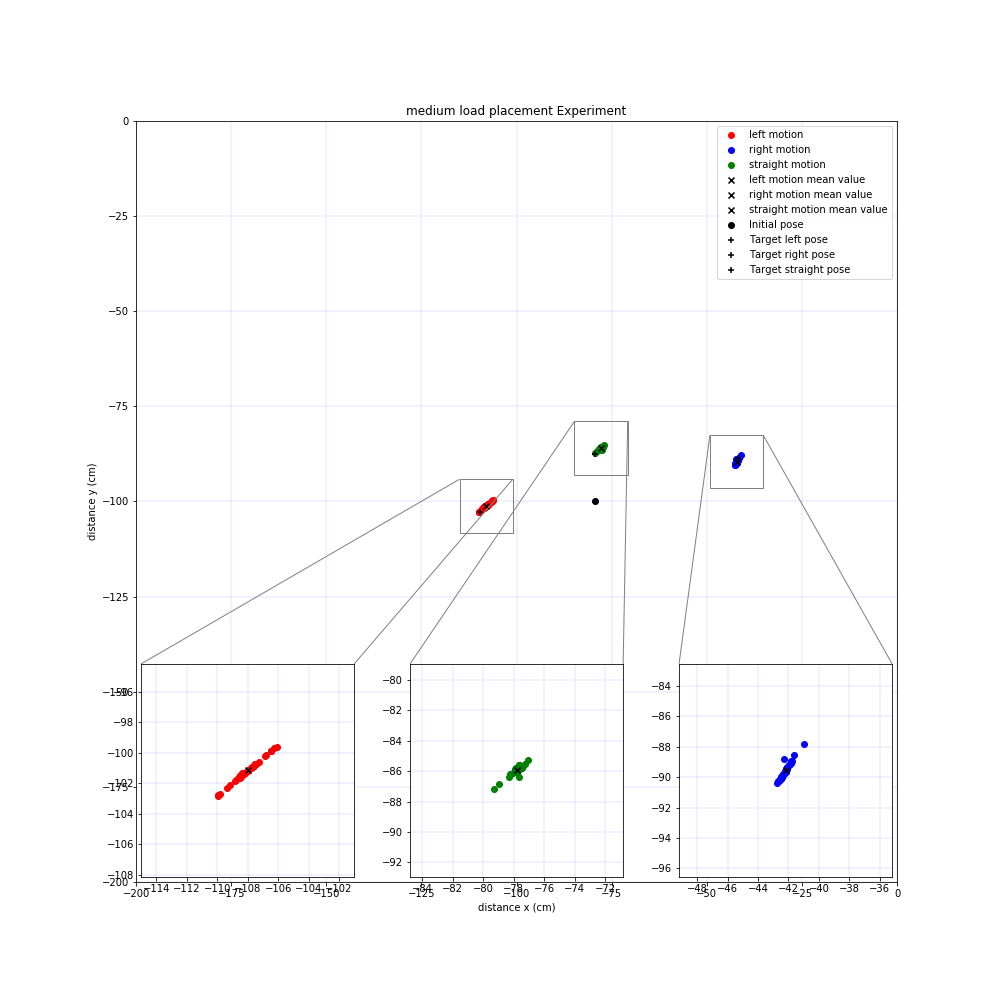
\includegraphics[width=0.6\linewidth]{images/combinedmedium}
	\caption{Results of the Medium Load Placement Experiment}
	\label{fig:combinedmedium}
\end{figure}
\begin{figure}[ht!]
	\centering
	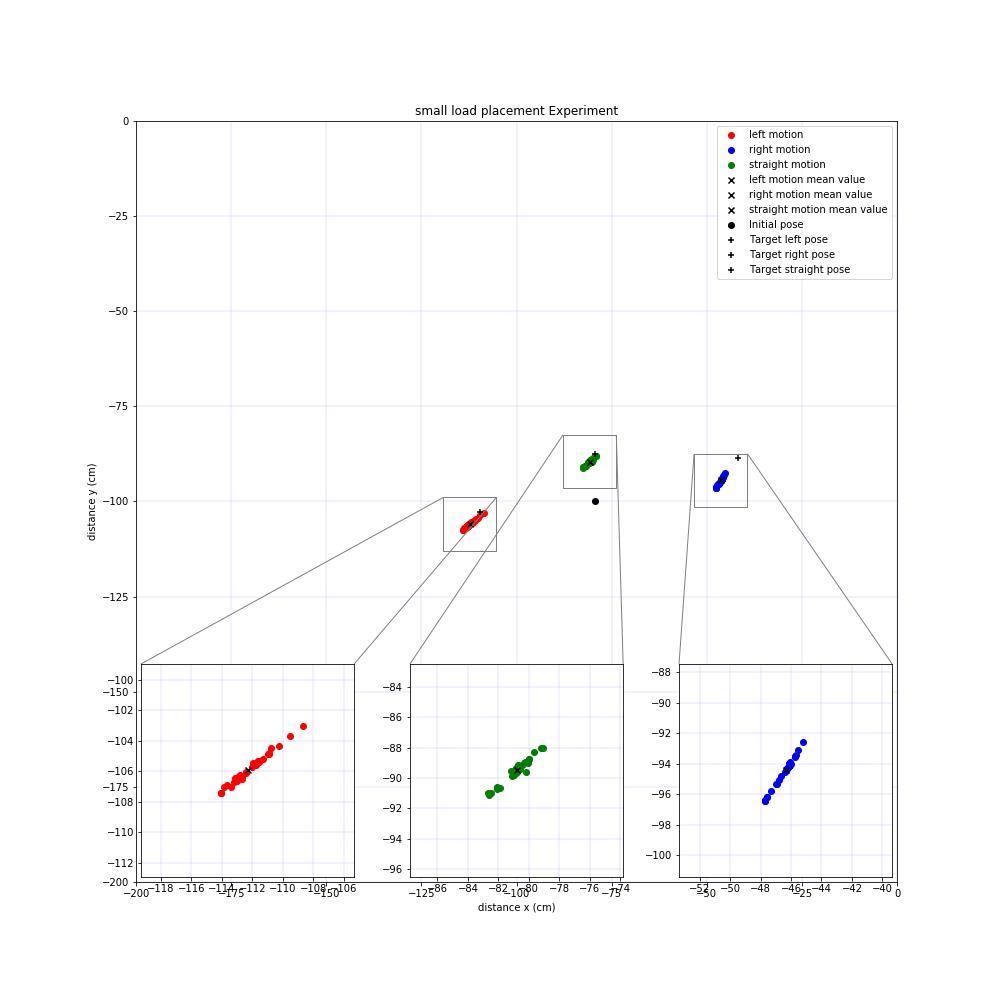
\includegraphics[width=0.6\linewidth]{images/combinedsmall}
	\caption{Results of the Small Load Placement Experiment}
	\label{fig:combinedsmall}
\end{figure}



%initial_pose = np.array([-79.27, -99.87, -1.62])
%target_straight = np.array([-79.40, -87.48, -1.72])
\newpage
\thispagestyle{empty}
{\footnotesize 
\begin{adjustbox}{angle=90}
	\centering
	\begin{tabular}{| l | c | c | c | c |c |c |c | c | c |}
		\hline
		                                                       &                  \multicolumn{3}{c|}{left}                   &               \multicolumn{3}{c|}{straight}               &                \multicolumn{3}{c|}{right}                 \\ \hline
		Our collected data                                     & big                & med                & small              & big               & med               & small             & big               & med               & small             \\ \hline
		target Pose $x$ cm       & -109.65& -109.65&-109.65 & -79.40 &-79.40 &-79.40 & -41.73 &-41.73 &-41.73 \\ 
		target Pose $y$ cm       & -102.75& -102.75&-102.75 & -87.48 &-87.48 &-87.48 & -88.63 & -88.63&-88.63 \\ 
		target Pose $\theta$ rad       & -2.10& -2.10& -2.10& -1.72 & -1.72& -1.72 & -0.92 &  -0.92& -0.92 \\ \hline
		uncertainty in pose $(\delta x \pm \sigma_x)$ cm       & $(-107.0 \pm 0.7)$ & $(-107.7 \pm 1.0)$ & $(-112.5 \pm 0.8)$ & $(-76.9 \pm 0.5)$ & $(-77.9 \pm 0.5)$ & $(-80.8 \pm 0.8)$ & $(-40.3 \pm 0.4)$ & $(-42.2 \pm 0.4)$ & $(-46.3 \pm 0.7)$ \\
		uncertainty in pose $(\delta y \pm \sigma_y)$ cm       & $(-99.5 \pm 0.6)$  & $(-100.9 \pm 0.8)$ & $(-106.1 \pm 0.7)$ & $(-84.4 \pm 0.4)$ & $(-86.0 \pm 0.4)$ & $(-89.4 \pm 0.7)$ & $(-87.1 \pm 0.8)$ & $(-89.5 \pm 0.6)$ & $(-94.3 \pm 1.0)$ \\
		uncertainty in pose $(\delta \theta \pm \sigma_y)$ rad & $(-2.1 \pm 0.0)$   & $(-2.1 \pm 0.0)$   & $(-2.1 \pm 0.1)$   & $(-1.6 \pm 0.1)$  & $(-1.6\pm 0.2)$   & $(-1.6 \pm 0.1)$  & $(-0.9 \pm 0.0)$  & $(-0.9 \pm 0.1)$  & $(-0.9 \pm 0.0)$  \\ \hline
		Combined Data                                          &                    &                    &                    &                   &                   &                   &                   &                   &                   \\ \hline
		uncertainty in pose $(\delta x \pm \sigma_x)$ cm       & $(-107.1 \pm 0.6)$ & $(-108.0 \pm 1.0)$ & $(-111.3 \pm 1.2)$ & $(-76.9 \pm 0.6)$ & $(-77.8 \pm 0.4)$ & $(-80.0 \pm 0.8)$ & $(-40.4 \pm 0.4)$ & $(-42.2 \pm 0.3)$ & $(-46.4 \pm 0.6)$ \\
		uncertainty in pose $(\delta y \pm \sigma_y)$ cm       & $(-99.6 \pm 0.5)$  & $(-101.2 \pm 0.9)$ & $(-106.0 \pm 1.0)$ & $(-84.4 \pm 0.6)$ & $(-86.0 \pm 0.3)$ & $(-89.5 \pm 0.7)$ & $(-87.3 \pm 0.7)$ & $(-89.6 \pm 0.5)$ & $(-94.4 \pm 0.9)$ \\
		uncertainty in pose $(\delta \theta \pm \sigma_y)$ rad & $(-2.1 \pm 0.0)$   & $(-2.1 \pm 0.0)$   & $(-2.1 \pm 0.1)$   & $(-1.6 \pm 0.1)$  & $(-1.6 \pm 0.1)$  & $(-1.7 \pm 0.2)$  & $(-0.9 \pm 0.0)$  & $(-0.8 \pm 0.1)$  & $(-0.9 \pm 0.0)$  \\ \hline
	\end{tabular}
	%\caption{Statistical summary of observed robot motion. Refer to Eq. \ref{mean-deviation}, \ref{standard-deviation}, \ref{mean-angular-deviation}. \update{Measurement uncertainty}}
	\label{stats}
\end{adjustbox}}
\newpage

\subsubsection{Knowing the ground-truth values of the expected final object poses, what is the accuracy of the arm? What about its precision?}
By observing the data, we can conclude that the arm provided is not accurate because of the large target end-effector pose error. But it is precise as the repeatability is high. 
  

\subsubsection{Does the distribution of the final object poses follow a Gaussian distribution?}

Yes, the distribution of the final poses follows a Gaussian distribution. 

\subsubsection{How much does changing the shape and mass of an object affect the final placing pose? Is this effect statistically significant? If the effects are indeed significant, what might have caused them? Hint: Statistical significance can only be determined by performing appropriate hypothesis tests.}

By observing the observed poses for big and small objects, for 60 samples for the hypothesis ``changing the shape and mass of an object affect the final placing pose", following results were obtained.

\vspace{0.5cm}

We consider $(2.5 cm, 2.5cm, 0.2 rad)$ as acceptable distance between two sampled points.\\
Average sampling error in hypothesis over observed data = 16. This is averaged value for running 100 random experiments. In each experiment, we took 20 samples for each motion movement.
\\
Hence,
\\
$$error_{S}(h) = \frac{1}{n} \times 16 = \frac{1}{60} \times 16 = 0.27$$

hence with approximately 95 $\%$ probability,
$error_{D}(h)$ lies in interval,

$$error_{D}(h) = \pm 1.96 \times \sqrt{\frac{error_{S}(h) \times (1 - error_{S}(h))}{n}} $$

$$error_{D}(h) = \pm 1.96 \times \sqrt{\frac{0.27 \times (1 - 0.27)}{60}} = \pm 0.11$$

Hence it can be concluded that above hypothesis holds true. 



\subsubsection{If we are to use a single camera measurement for determining the final object pose instead of multiple filtered measurements, is the effect on the final pose estimates significant?}

By observing the observed poses for big and small objects, for 60 samples for the hypothesis ``Using single camera measurement does not affect the final object pose measurement", following results were obtained.

\vspace{0.5cm}
We consider $(1.0 cm, 1.0cm, 0.1 rad)$ as acceptable distance between two sampled points.\\
Error in hypothesis over observed data = 0
\\
Hence,
\\
$$error_{S}(h) = \frac{1}{60} \times 0 = 0.0$$

hence with approximately 95 $\%$ probability,
$error_{D}(h)$ lies in interval,

$$error_{D}(h) = \pm 1.96 \times \sqrt{\frac{error_{S}(h) \times (1 - error_{S}(h))}{n}} $$

$$error_{D}(h) = \pm 1.96 \times \sqrt{\frac{0.0 \times (1)}{60}} = \pm 0.0$$

Hence it can be concluded that above hypothesis holds true. 

Though, a situation could occur where because of some environmental uncertainties, pose estimated by camera in one frame is deviated significantly and that pose is used in experimentation. This can introduce a significant error. 

\subsection{Mention the list of used software and include the source of any functions you wrote for performing your analysis.}
\begin{itemize}
\item We output generated by \texttt{Subscriber.py} was a broken \texttt{json} file. Therefore importing the data was non-trivial. We wrote a \texttt{runscripts.sh} bash script that was a workaround to search for the relevant data from all the recordings and then write it to \texttt{csv} files.
\item The \texttt{runscripts.sh} requires \texttt{read.py} as dependency file.
\item Each data point was collection of 50 poses $(x, y, \theta)$. This was done to add redundancy such that the measurement is tolerant to measurement-faults. The \texttt{runscripts.sh} file already take the mean value of these readings and writes the mean value to respective \texttt{csv} file.
\item All the data stored in \texttt{csv} files is then imported to a \texttt{jupyter notebook} for plotting and statistical analysis.
\item All the code is attached alongside with the submitted report.
\end{itemize}

%%%%%%%%%%%%%%%%%%%%%%%%%%%%%%%%%%%%%%%%%%%%%%%%%%%%%%%%%%%%%%%%%%%%%%%%%%%%%